

\chapter{State of the Art}
\label{sec:sota}

Forest fire occurrence prediction is a crucial task for lessening the impact of wildfires on the environment, economy, and human health. Various factors, such as weather, topography, vegetation, and human activities, influence the likelihood and frequency of fire ignition and spread. To model and map these factors, different mathematical and machine learning techniques have been proposed and applied in the literature. 


This chapter reviews the state of the art methods for forest fire occurrence, susceptibility, and risk prediction, as well as the data sources, tools, and challenges involved in this task.


At last, it is addressed methodologies and techniques for data aggregation, fusion, and enhancement and data visualisation tools.


\section{Importance of Machine Learning in Forest fire prediction}
Machine learning algorithms have the ability to automatically anticipate and identify fire incidents \cite{Abid2021}. They are able to simulate how fire danger is influenced by variables like topography and weather. 


Wildfire occurrence prediction will often take multiple approaches to decision-making by utilising multiple machine learning models in conjunction with mathematical models. This aids in predicting the likelihood and risk of a forest fire spreading before it starts \cite{Abid2021}. Additionally, machine learning models are also capable of predicting the behaviour of forest fires, or the development of their spread \cite{Abid2021}.


Taking \gls{cnn} and other machine learning models as an example, these models have been used to conduct spatial prediction of forest fire susceptibility \cite{zhang2019forest}. 


Predicting fire risks is crucial to minimize monthly fire emissions across large regions and reduce the consequences of fires on human health, air quality, and climate change \cite{wang2022interpreting}. Machine learning models can help local authorities and fire services use their resources more wisely in addition to averting disasters and saving lives in the event of a fire \cite{surya2017risk}.


\section{Mathematical models in forest fire prediction}

Sometimes machine learning models are assembled in conjunction with mathematical models. These models estimate the chance and probability of a forest fire occurrence using functions and algorithms. Some models can rely on meteorological characteristics such as temperature, humidity, wind speed, and rainfall to forecast forest fires. The most famous mathematical model is the \gls{fwi}. 


The canadian FWI and other forest weather systems give numerical indices for predicting and avoiding fires. It is a technique for calculating indices based on temperature, relative humidity, rain, and other variables \cite{mohammed2020comparative}. This rating incorporates the chance of fire ignition and the pace of fire spread \cite{doi:10.1155/2014/597368}. This approach is employed not just in Canada, but also in various European nations, like Portugal \cite{mohammed2020comparative}. 


Another example is the Angstrom index, which is a basic fire index that calculates the likelihood of a fire depending on relative humidity and temperature. It was created in Sweden and is used in some regions of Scandinavia to predict when fires will start on a particular day \cite{land12010194}. 


Some models discussed in the state of the art will even tackle the \gls{kbdi}, which is a tool that assesses drought conditions. It is frequently applied to forecast the probability and intensity of wildfires \cite{KBDI}.

\section{Influencing factors}
\label{influencing_factors}

Forest fires require an ignition triangle of oxygen, heat source, and fuel, which can be found in trees, grasses, dry bushes, and forest litter. Lightning, scorching winds, and even the sun are the most common natural sources of ignition \cite{rs13132513}. 


Influencing factors regarding wildfires can be split into two main categories of risk: Long-term risk that is defined by the components of a territory that do not vary over the long term such as landscape factors and population factors. Short-term risk is defined by factors that change, such as weather conditions and temporal factors \cite{Novo2020MappingFF}.


The following list will encompass the main factors concerning wildfire incidence:
\begin{itemize}
    \item Weather factors: temperature, humidity, wind speed, precipitation, relative humidity, water vapour pressure, thunderstorms, rainfall, oxygen, CO level \cite{10085661, arif2021role, Sharma2020, f14020170};
    \item Temporal factors: season, month, time of day \cite{arif2021role};
    \item Population factors: population density, human activities in the forest, human behaviour, short circuits in power lines that cross the forest \cite{arif2021role};
    \item Landscape factors: tree types, slope, distance from agricultural lands, road distance, settlement distance, fuel mode types, vegetation, topography \cite{Novo2020MappingFF, arif2021role, bountzouklis2023predicting}.    
\end{itemize}



\section{Forest fire occurrence prediction}
Estimating how many and where fires may occur in the next days is essential to making advance plans for dealing with fire crises. Numerous variables, including the weather, lightning, and other elements impact the risk of fire and influence prediction (see section \ref{influencing_factors} for a more complete list of factors regarding fire ignition and spread). 

Forest fire occurrence models utilize statistical methods and machine learning to establish a relationship between an output (such as fire reports or hotspots) and influencing factors. This relationship is used to predict the likelihood of forest fires in specific regions or geographical areas \cite{jain2020review}.

\subsection{Decision tree}
The authors of \cite{abid2020predicting} presented an algorithm that uses a decision tree classifier and meteorological data to forecast the likelihood of forest fires in Algeria. The input elements were temperature, relative humidity, wind speed, and rain. 


The output classifications included fire and non-fire. The model yielded an accuracy of 82.92\% and a recall of 0.92 for the fire class when tested on a dataset gathered from two areas in Algeria.


\subsection{Random Forest Algorithm}
The study shown in \cite{9726029} investigated the influence of various factors such as humidity, temperature, wind speed, and rain using a hybrid approach with a random forest algorithm and components like \gls{ffmc}, \gls{dmc}, \gls{dc}, and \gls{isi} from the fire weather index.
The study made use of a dataset gathered over three years, from January 2000 to December 2003, from the Montesinho natural park in Trás-os-Montes \cite{misc_forest_fires_162}.


A correlation matrix was utilised and indicated that temperature, month, FFMC, DMC, DC, and ISI are directly related or proportional, while rain and temperature show no correlation. The random forest regression model obtained a mean absolute error of 0.6664 and a regression score of 0.9799, which means the model can explain 97.99\% of the variation in the data.

The confusion matrix showed that the model could correctly classify most of the samples as fire or no fire. The paper addressed the fact that weather forecasting is useful to predict favourable climatic conditions for wildfire occurrences.


\subsection{Boosted Decision trees}
The paper "A smart approach for fire prediction under uncertain conditions using machine learning" \cite{Sharma2020} conducted an experiment on the \cite{misc_forest_fires_162} dataset with 8 different classification models, and out of them, boosted decision trees had the highest \gls{auc} value. Results containing the comparison between the classification models can be seen in table \ref{cortez_classification_results}.

\begin{table}[h!]
\caption{Classification models results on \cite{misc_forest_fires_162} dataset.}
\begin{tabular}{|l|l|l|l|l|l|}
\hline
\textbf{Algorithm} & \textbf{Precision} & \textbf{Recall} & \textbf{F-score} & \textbf{Accuracy} & \textbf{AUC} \\ \hline
Boosted Decision Trees & 76\% & 76\% & 76\% & 72\% & 0.787302 \\ \hline
Decision Forest Classifier & 75\% & 71\% & 73\% & 69\% & 0.753968 \\ \hline
Decision Jungle Classifier & 70\% & 80\% & 75\% & 69\% & 0.752381 \\ \hline
Averaged Perceptron & 67\% & 90\% & 77\% & 69\% & 0.634921 \\ \hline
2 Class Bayes Point Machine & 60\% & 80\% & 69\% & 58\% & 0.514286 \\ \hline
Local Deep SVM & 81\% & 61\% & 70\% & 69\% & 0.68254 \\ \hline
Logistic Regression & 60\% & 100\% & 75\% & 69\% & 0.749226 \\ \hline
Binary Neural Network & 60\% & 70\% & 64\% & 63\% & 0.69969 \\ \hline
\end{tabular}

\label{cortez_classification_results}
\end{table}

\subsection{Logistic Regression}
The authors of \cite{10085661} used a logistic regression model and concluded that there were only three variables: humidity, temperature, and oxygen. It was possible to conclude that high humidity and low temperatures are correlated with a low probability of fire occurrence. The model obtained on the test dataset achieved an accuracy of 93.75\%, a precision of 94.12\%, a recall of 93.75\%, and an F1-score of 93.94\%.

\subsection{ANN}
\gls{ann} are statistical models that draw inspiration from biological neural networks and are partially based on them. They are able to represent and handle nonlinear interactions between inputs and outputs. The linked algorithms can be applied in a variety of ways and are a component of machine learning \cite{al2021predicting}.

\subsubsection{Comparing ANN and SVM}
\label{ComparingANN_SVM}
A unique approach for creating a dataset based on data from remote sensing and data mining algorithms to forecast the incidence of wildfires was suggested by \cite{SAYAD2019130}. Big data, remote sensing and data mining algorithms were combined to process data collected from satellite images and extract insights to predict the occurrence of wildfires.


The dataset includes three factors relating to crop health, soil temperature, and fire indicators that were retrieved from \gls{modis} tools. It consists of 804 cases from various zones in the centre of Canada, mostly in British Columbia and Quebec, where wildfires had previously occurred.


ANNs and \gls{svm} were employed as data mining methods. According to the study, the suggested model performs better than other models in terms of sensitivity, specificity, precision, and F-score and achieves high accuracy (98.32\% for neural networks and 97.48\% for SVM). 


The table \ref{arima} shows the comparison of results between the different models, STIFF and ISTFF are frameworks mentioned in other papers, that were compared to the solution proposal of \cite{SAYAD2019130}.


\begin{table}[h!]
\caption{Results comparison between ANN and other models}
\centering
\begin{tabular}{|l|l|l|}
\hline
\textbf{Model} & \textbf{Accuracy} & \textbf{RANK} \\ \hline
ARIMA & 83.5\% & 4 \\ \hline
STIFF & 65\% & 5 \\ \hline
ISTFF & 95\% & 3 \\ \hline
ANN & 98.32\% & 1 \\ \hline
SVM & 97.48\% & 2 \\ \hline
\end{tabular}
\label{arima}
\end{table}


\subsubsection{ANN with KBDI}
The authors of \cite{sadatrazavi2022predicting} developed a novel model for forecasting wildfires using meteorological parameters and ANNs. A wildfire database was gathered from the \gls{usda}, and the \gls{ecmwf} provided satellite data for the model's inputs and outputs. 


The inputs include temperature, relative humidity, total pressure, evaporation, soil moisture, snow storage, precipitation, wind speed, \gls{ndvi}, and the Keetch-Byram drought index. The outputs consist of two values: one (1) for wildfire incidences and zero (0) for records that do not include a fire.

The study made conclusions about the factors influencing fire ignition for temperate forests and boreal forests. It concluded that while precipitation was also significant for boreal forests, the most significant factors for both types of forests were determined to be relative humidity, total pressure, wind speed, and KBDI.






\subsection{Explainable Artificial Intelligence (XAI)}
\gls{xai} approaches are utilised to determine which factors contribute most substantially to the occurrence of wildfires while making models more interpretable for stakeholders. In this regard, the paper "Predicting wildfire ignition causes in Southern France using eXplainable Artificial Intelligence (XAI) methods" \cite{bountzouklis2023predicting} used an explainable artificial intelligence framework to classify the source of fire ignition based on environmental and anthropogenic variables. 


This study aimed to determine if the sources of unknown-caused fires could be predicted using machine learning. The study's results explained that natural fire prediction accuracy (F1-score 0.87) is higher than human-caused fire prediction, such as accidental (F1-score 0.74) and arson (F1-score 0.64) \cite{bountzouklis2023predicting}. While this study does not focus entirely on the spatial and temporal prediction of wildfire occurrences, it is worth quoting the feasibility of a method like this for the study of wildfire forecasting.





\section{Forest fire susceptibility prediction}

Creating susceptibility maps from forest fire occurrence prediction is a technique for identifying regions prone to forest fires. It is concerned with the prospect of harm to human health and property, as well as environmental health and its potential implications. This is accomplished by examining the many elements that contribute to the chance of a fire happening in a certain location, as well as the dependency relationships between the components. These components can be both natural and produced by humans \cite{Sevinç2023}.

\subsection{BRT, GLM and MDA}


The authors of \cite{POURGHASEMI2020109321} developed forest fire susceptibility maps from Landsat-8 \gls{oli} and MODIS satellite photos from 358 sites in Fars Province, Iran, using three machine-learning approaches to examine the determinants and spatial patterns of forest fire susceptibility.


Elevation, slope, topographical wetness index, aspect, distance from metropolitan areas, annual mean temperature, land usage, distance from the road, annual mean rainfall, and distance from the river were recognised as the 10 most important feature for fire susceptibility. 


The geographical correlations between the 358 historical fire sites and the 10 contributing factors were analysed using the \gls{brt}, \gls{glm}, and \gls{mda}. Various criteria, such as the ROC curve, accuracy, overall accuracy, and \gls{tss}, were used to assess prediction accuracy. These three models provide a forest fire susceptibility map with four risk levels: very high, high, moderate, and low.


The study discovered that among the three models, BRT had the best prediction accuracy (AUC = 0.882) and the lowest standard error, followed by MDA (AUC = 0.856) and GLM (AUC = 0.825). The researchers also employed \gls{lvq} to determine the relative relevance of the contributing elements, and they discovered that land use, annual mean rainfall, and slope were the most important determinants for forest fire vulnerability.


According to the study, the BRT and MDA models were adequate and trustworthy for mapping forest fire susceptibility in Fars Province, and the produced maps might aid in the planning and management of forest resources and ecological balances.







\section{Forest fire risk prediction}
Forest fire risk assessment is a scientific process for quantifying risk levels, allowing decision-makers to weigh the benefits and drawbacks of various measures. It includes data about the likelihood and extent of future forest fires based on current fire behaviour such as ignition, spread, suppression, and longevity \cite{rs13132513}.

Forest fire risk assessment can be split into four stages \cite{rs13132513}: 
\begin{enumerate}[label=(\alph*)]
    \item identification of hotspot locations;
    \item calculation of forest fire susceptibility;
    \item identification of forest fire sensitive areas;
    \item assessment of likely forest fire risk.
\end{enumerate}


\subsection{Multilayer perceptron and Fuzzy logic supervised approach}
The authors of \cite{rs13132513} developed a solution to output a risk index in a geographical area near Sydney, Australia. The risk was determined by a combination of three factors: social vulnerability, physical vulnerability, and a hazard index.
Social and physical vulnerability were computed given a set of social and demographical features. While the hazard index was created given a combination of forest fire influencing factors (such as NDVI, slope, rainfall, temperature, and land cover) and fire ignition points, These two elements contributed to the creation of the susceptibility map. The ignition points were based on a historical inventory database of Australian forest fire ignition spots.


The susceptibility model for the harzard index was made with a multilayer perceptron model, which consists of multiple layers of neurons connected by weighted links \cite{bento2020multilayer}.


The model was then optimised using a \gls{fbsp} to find the best values for the hyper-parameters.

The result of the study can be seen in Fig. \ref{fig:ffrpm}, where a map for forest fire risk is shown.

\begin{figure}[htbp]
 \centering
  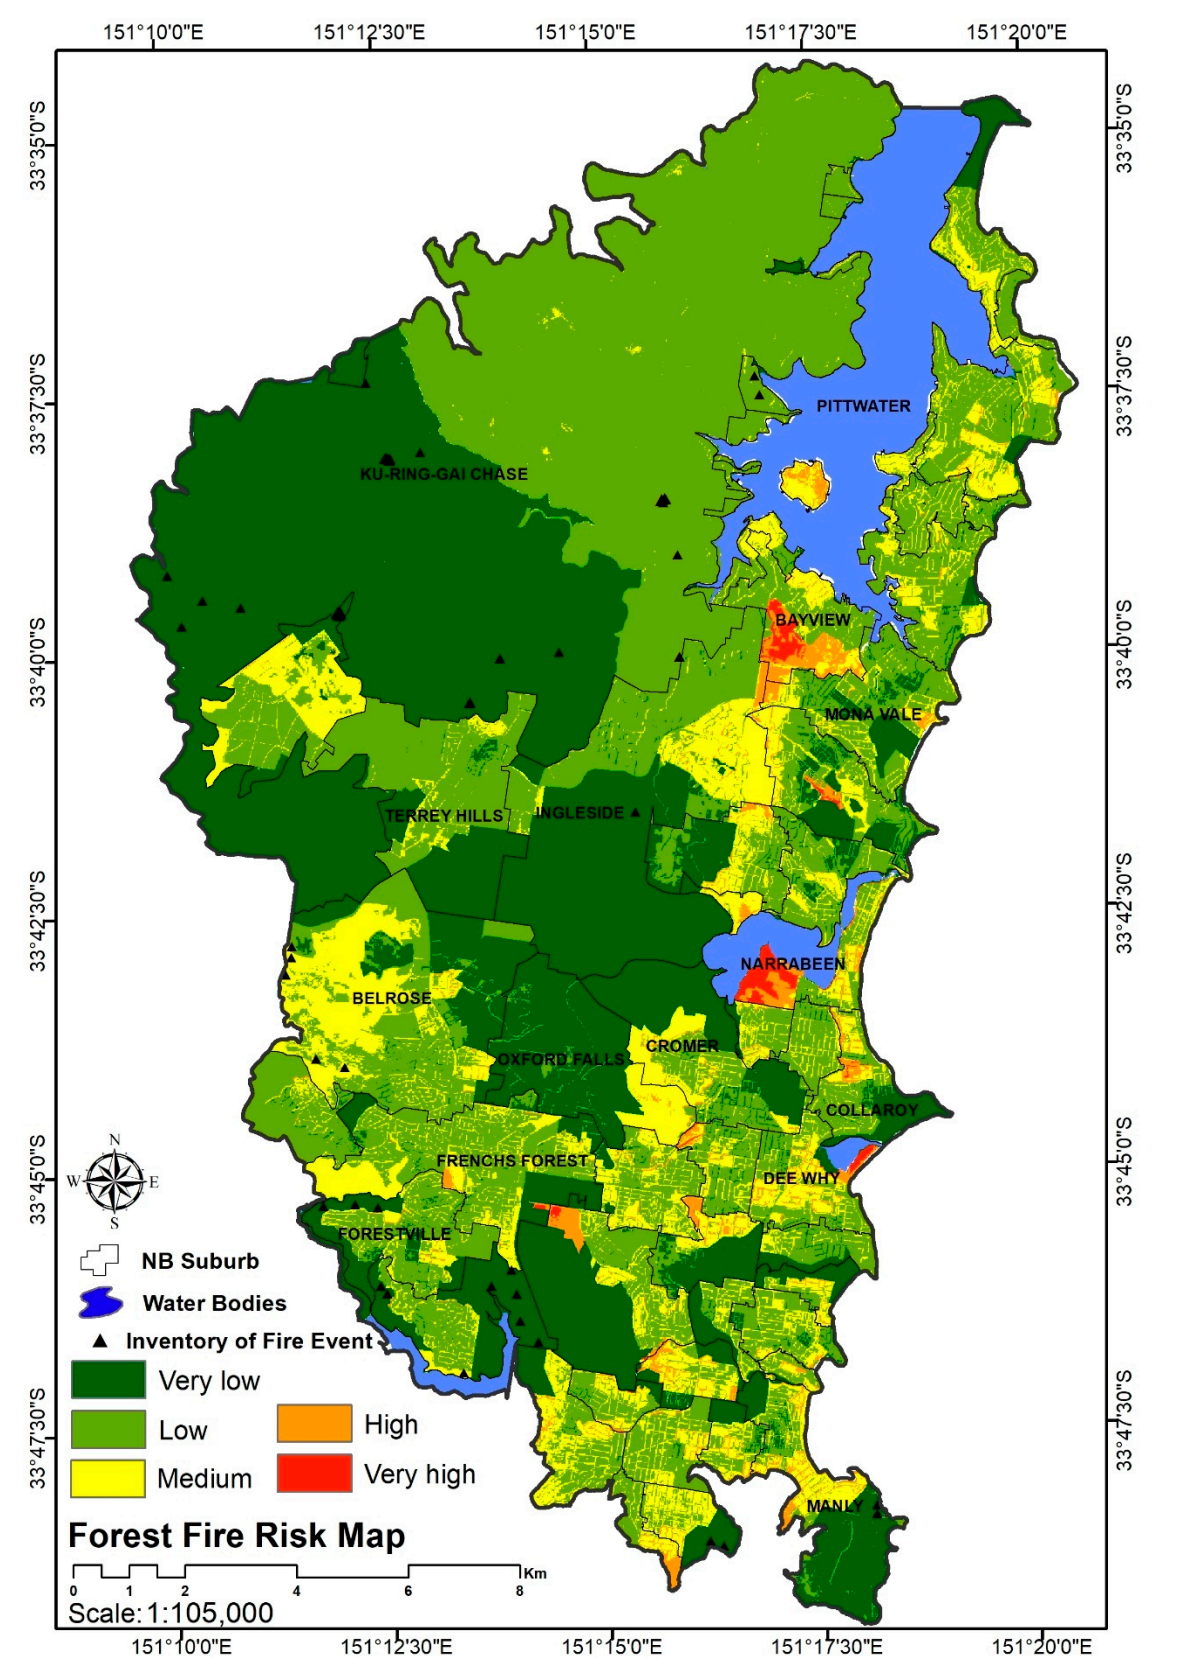
\includegraphics[width=0.4\linewidth]{frontmatter/imgs/Screenshot from 2023-11-28 11-07-47.png}
  \caption{Forest fire risk map}
  \label{fig:ffrpm}
\end{figure}



\subsection{Ant-miner algorithm}
A study conducted by \cite{ZHENG2020106772} mined decision rules using historical fire data and risk factor data from Chongqing, China. The authors stated risk factor data as a combination of the following parameters:
\begin{itemize}
    \item Meteorological data: wind speed, air temperature, relative humidity, accumulated precipitation, continued non-precipitation days;
    \item Land cover data: land cover type;
    \item human activity data: distance from nearest road and residential area.
\end{itemize}
An ant-miner algorithm was used to mine decision rules from the data and forecast the danger level of forest fire across the study region. A confusion matrix was also used in the study to assess the accuracy of the proposed model, which was then compared to existing models such as artificial neural networks, and support vector machines. 


The model was also compared to a risk prediction model based on meteorological data that calculated a \gls{ffdwi} according to China's national standard using five meteorological factors (wind speed, air temperature, relative humidity, accumulated precipitation, and continuous non-precipitation days). 


Another risk prediction model was based on the artificial neural network (ANN) technique, which employed the same risk elements (meteorological data, land cover data, and human activity data) to train a multilayer perceptron network for forecasting the risk level of forest fire. A support vector machine (SVM) was used and employed the same risk parameters as the proposed model to train a kernel-based classifier for predicting the risk level of forest fire.


The model's performance was compared using a confusion matrix. In terms of overall accuracy and Kappa coefficient, the ant-miner model surpassed the others.




The study acknowledged that the proposed model may lack generalisability across different geographical locations and may be unable to describe the risk distribution of forest fires as a specific mathematical function when multiple factors' joint probability distribution functions are considered.


\subsection{Fuzzy Inference}
The authors of \cite{LIN2018101} offer a novel approach for predicting and assessing forest fire risk using fuzzy inference (the process of applying fuzzy logic to create a mapping from a given input to an output \cite{KALOGIROU2009553}), and large data analysis. Figure \ref{fig:fuzzy_risk_prediction} explains visually the basic logic of the approach.


The project was built with a \gls{rwsn} in mind that is collecting continuous 24-hour meteorological data, and installed in a forest region in the Nanjing City region of China. Temperature, humidity, wind speed, rainfall, season, date, time, historical fire data, population density, fuel type, and road density are all input parameters.

\begin{figure}[h!]
 \centering
  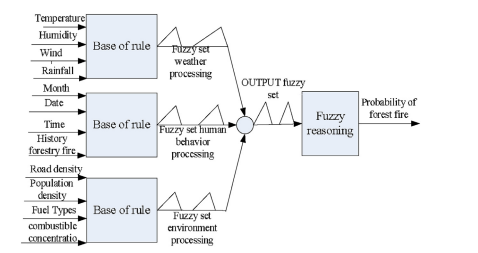
\includegraphics[width=0.7\linewidth]{frontmatter/imgs/fuzzy_prediction_model.PNG}
  \caption{Prediction of forest fire risk using a fuzzy reasoning algorithm \cite{LIN2018101}.}
  \label{fig:fuzzy_risk_prediction}
\end{figure}


The method generates the fire rating output by using triangular fuzzy numbers to reflect the uncertainty and ambiguity of the input parameters. The output fire rating is divided into five categories: low, moderate, high, very high, and extreme.
It was concluded that the system can accurately forecast possible fire danger and provide helpful information for forest fire prevention and management. Figure \ref{fig:prediction_graph_fuzzy} depicts fire probability given the oscillation of influencing factors. 

\begin{figure}[h!]
 \centering
  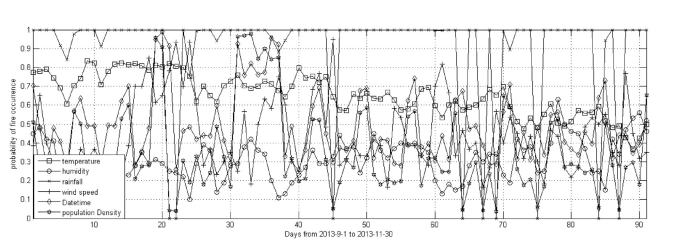
\includegraphics[width=1\linewidth]{frontmatter/imgs/p_ocurrencia_incendio.PNG}
  \caption{Meteorological data, datetime, and people density to predict the likelihood of a forest fire \cite{LIN2018101}.}
  \label{fig:prediction_graph_fuzzy}
\end{figure}



\subsection{Auto-sklearn}
An autonomous machine learning framework for forecasting the danger of forest fires based on meteorological data was proposed by \cite{Qu_2020}. This framework is capable of adapting to varied datasets and geographies. When it comes to binary unbalanced datasets, the machine learning techniques currently in use for forest fire prediction are not very compatible. 


The dataset used in the article comes from Montesinho Nature Park \cite{misc_forest_fires_162} and contains historical data about fire occurrences in the place. The framework optimises auto-sklearn, in terms of data preprocessing, parameter learning, and loss function.


The experimental findings demonstrated that the framework has strong geographic flexibility and performs better than other state-of-the-art machine learning techniques. Table \ref{sklearnpro} illustrates how Auto-Sklearn Pro performs better than other models when meta-learning is modified and a new bayesian optimisation index is included.




\begin{table}[h!]
\caption{Forest district classifier accuracy comparison}
\centering
\resizebox{\textwidth}{!}{%
\begin{tabular}{|c|c|c|c|}
\hline
\textbf{Forest District} & \textbf{Classifier} & \textbf{Accuracy (Overall)} & \textbf{Accuracy (Minority sample)} \\
\hline
District1 & AUTO-SKLEARN PRO & 87.3\% & 94.2\% \\
 & AUTO-SKLEARN & 86.4\% & 72.5\% \\
 & SVM & 84.6\% & 67.3\% \\
 & RandomForest & 75.5\% & 69.2\% \\
 & AUTO-SKLEARN PRO & 85.6\% & 90.4\% \\
\hline
District2 & AUTO-SKLEARN & 89.5\% & 74.3\% \\
 & SVM & 82.3\% & 63.2\% \\
 & RandomForest & 71.1\% & 73.0\% \\
 & AUTO-SKLEARN PRO & 82.4\% & 87.1\% \\
\hline
District3 & AUTO-SKLEARN & 85.3\% & 79.8\% \\
 & SVM & 73.1\% & 54.4\% \\
 & RandomForest & 69.5\% & 72.1\% \\
\hline
\end{tabular}%
}

\label{sklearnpro}
\end{table}


\subsection{DFP-MnBpAnn}
The authors behind \cite{TIENBUI2018104} proposed DFP-MnBpAnn, a new hybrid machine learning technique for spatial modelling of forest fire threat based on Artificial Neural Network (Ann) and a unique hybrid training algorithm of Differential Flower Pollination (DFP) and mini-match backpropagation (MnBp). 


Flower Pollination technique is a a nature-inspired, metaheuristic optimisation technique that mimics flower pollination. Solutions are viewed as flowers in FPA, and the process of identifying the optimum solution is analogous to pollination. 


Differential Evolution (DE), on the other hand, is a population-based optimisation technique that employs the evolutionary notion. It begins with a randomly generated population of solutions and improves them repeatedly using mutation, crossover, and selection procedures. 


The two algorithms are merged in such a way that they compliment each other in a hybrid training algorithm of DE and FPA \cite{Abdel-Basset2019}. 

\begin{figure}[h!]
 \centering
  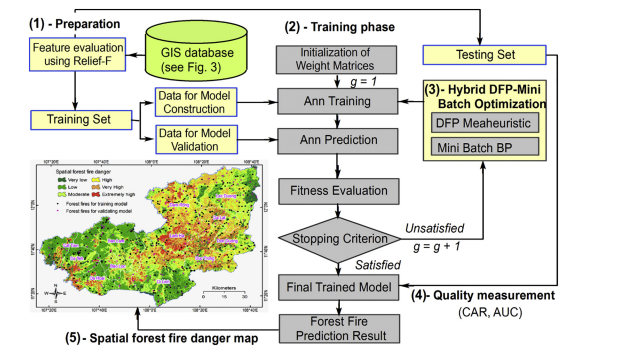
\includegraphics[width=1\linewidth]{frontmatter/imgs/hybrid_methodology.PNG}
  \caption{Methodology used with DFP-MnBpAnn\cite{LIN2018101}.}
  \label{fig:hybrid:dfpann}
\end{figure}

The factors influencing forest fire were slope, aspect, elevation (m), land use, NDVI, distance to road (m), distance to residential area (m), temperature (°C), wind speed (m/s), and rainfall (mm). They were generated from GIS data (see Figure \ref{fig:hybrid:dfpann} for a complete view of the proposed framework) to apply the suggested strategy to a tropical forest in Vietnam's Lam Dong province. 


The DFP-MnBpAnn model outperformed the other six approaches in terms of prediction accuracy (88.43\%) and AUC (0.94), highlighting its superiority and promise for large-scale forest fire threat mapping. The table \ref{table_dfp} presents the complete results of DFP-MnBpAnn's performance metrics against other models.


\begin{table}[h!]
\caption{DFP-MnBpAnn performance metrics against other prediction models \cite{TIENBUI2018104}}
    \centering
    \begin{tabular}{lccccccc}
        \hline
        \multirow{2}{*}{Phase} & \multirow{2}{*}{Model} & \multicolumn{6}{c}{Performance Metrics} \\
        \cline{3-8}
         & & CAR (\%) & AUC & TP & FP & FN & TN \\
        \hline
        \multirow{6}{*}{Training} & DFP-MnBpAnn & 87.30 & 0.91 & 0.94 & 0.20 & 0.06 & 0.80 \\
         & PSO-NF & 89.30 & 0.93 & 0.96 & 0.17 & 0.04 & 0.83 \\
         & RF & 86.40 & 0.91 & 0.91 & 0.19 & 0.09 & 0.81 \\
         & SVM & 86.20 & 0.89 & 0.92 & 0.19 & 0.08 & 0.81 \\
         & LSSVM & 86.24 & 0.89 & 0.90 & 0.18 & 0.10 & 0.82 \\
         & BpAnn & 89.02 & 0.94 & 0.93 & 0.15 & 0.07 & 0.85 \\
        \hline
        \multirow{6}{*}{Testing} & DFP-MnBpAnn & 89.20 & 0.94 & 0.94 & 0.15 & 0.06 & 0.85 \\
         & PSO-NF & 85.80 & 0.92 & 0.92 & 0.20 & 0.08 & 0.80 \\
         & RF & 85.20 & 0.91 & 0.90 & 0.19 & 0.10 & 0.81 \\
         & SVM & 84.90 & 0.88 & 0.88 & 0.19 & 0.12 & 0.81 \\
         & LSSVM & 86.42 & 0.88 & 0.92 & 0.19 & 0.08 & 0.81 \\
         & BpAnn & 85.03 & 0.89 & 0.91 & 0.21 & 0.09 & 0.79 \\
        \hline
    \end{tabular}
    \label{table_dfp}
\end{table}


\section{Methodologies for data aggregation, fusion, and enhancement}
\subsection{Data aggregation}
The process of merging information from several sources into a single dataset is known as data aggregation. These sources may consist of databases, sensor networks, or other types of data repositories containing Weather, location, and historical fire event data \cite{Cai2019}. Data aggregation can be split into two key-categories \cite{papvco2021fusion}:
\begin{itemize}
    \item Temporal aggregation: Combining data across predetermined time frames. Finding trends linked to fire seasonality, such as daily meteorological data that may be combined to produce monthly or seasonal averages \cite{papvco2021fusion}.
    \item Spatial aggregation: Combining data across geographic regions. This can aid in comprehending how fire risk elements are distributed spatially \cite{papvco2021fusion}.
\end{itemize}

\subsection{Data fusion}
\label{data_fusion}
Data fusion refers to the need to combine information obtained from many sources (sensors, databases, information gathered by people, apis) in order to present complementary interpretations of the same phenomenon. It provides more exact results than those obtained by using a single dataset, eliminating ambiguity and redundancy. \cite{CHATZICHRISTOS2022341, LACROIX200375}

Figure \ref{fig:meth:data_fusion} describes visually two data fusion techniques that will be utilised. The following list explains each one:
\begin{itemize}
    \item Decision-Level fusion: In this technique, characteristics are extracted from the data and one or more intermediate analyses are carried out until an appropriate result for the problem is achieved \cite{articleDataFusion}.
    \item Feature-level fusion: This technique involves collecting features from each data source and then merging them \cite{articleDataFusion}.
\end{itemize}

\begin{figure}[h!]
 \centering
  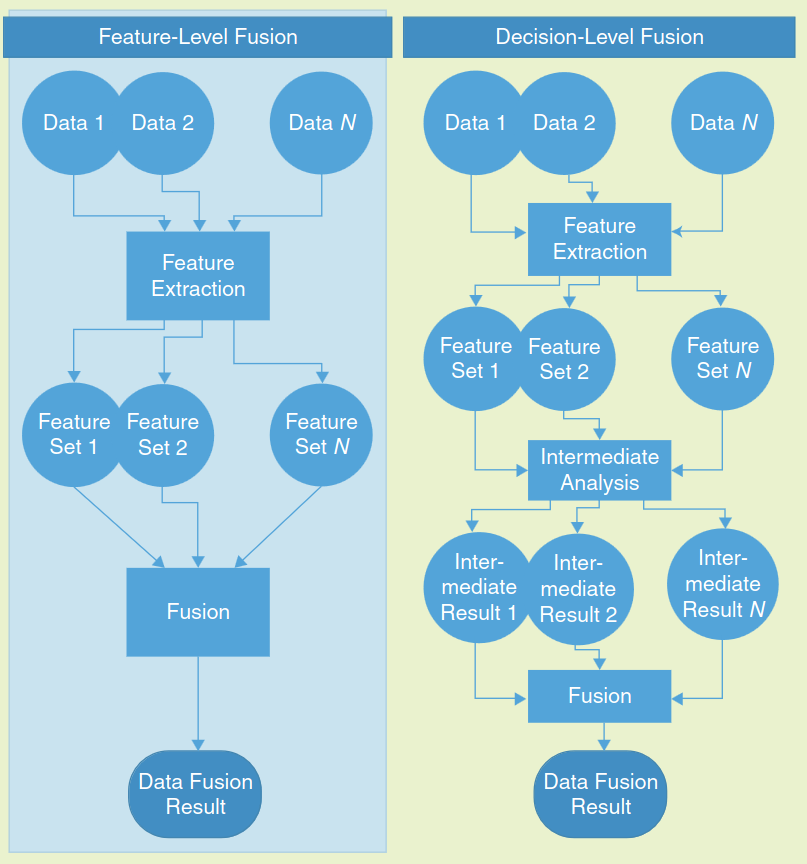
\includegraphics[height=0.7\linewidth]{frontmatter/imgs/ffdf2.png}
  \caption{Methodologies for Data fusion \cite{articleDataFusion}.}
  \label{fig:meth:data_fusion}
\end{figure}

\subsection{Data enhancement} 
The process of changing, converting, or adding to data in order to make it better and easier to use is known as data enhancement \cite{clickworker2021}. 
It can be achieved by using multiple paths such as:
\begin{itemize}
    \item Data Enrichment: Using numerous third-party data to supplement the original data \cite{mparticle_data_enrichment}.
    \item Synthetic Data Generation: Created artificially without utilising the original dataset \cite{awan2023complete_guide_data_augmentation}.
\end{itemize}



\section{Tools for data visualization}

\subsection{Seaborn}
\label{dv_seabon}
Seaborn is a high-level interface for creating visually appealing statistical visuals and is developed on top of Matplotlib, which is a charting toolkit and allows the creation of all kinds of plots and charts \cite{seaborn}\cite{matplotlib}.

\subsection{Folium}
Folium is a Python wrapper for Leaflet.js map tool. It helps in spatial data visualisation \cite{folium}.

\subsection{GeoPlot}
It is based on Matplotlib and GeoPandas. Geoplot offers a high-level mapping creation interface. GeoPandas is a library extension for Pandas that facilitates mapping and has geographic functions. It manages and produces maps using geospatial data \cite{geoplot, geopandas, matplotlib}.

\subsection{Plotly}
\label{dv_plotly}
Plotly is a robust and interactive charting library. It works with many different kinds of charts and is helpful for making interactive visualisations. \cite{plotly}.

\subsection{Rasterio}
Rasterio is used to read and write geographic raster data, such as satellite images. \cite{rasterio}.

\subsection{Pydeck}
Pydeck is a WebGL-powered, high-layer framework that is used to create dynamic maps covering sizable regions \cite{pydeck}.

\subsection{Rasterstats}
Geospatial raster datasets may be summarised using rasterstats based on vector geometry. It is also used to compute statistics within certain regions \cite{rasterstats}.

\subsection{Fiona}
The goal of Fiona is to simplify the reading and writing of geographic data files. It makes dealing with vector data easier and is based on GDAL which is a potent open-source library for reading and writing geographic data formats in both raster and vector forms. \cite{fiona, gdal}.


\section{State-of-the-art conclusion}

Throughout this chapter, various methodologies for predicting occurrence, susceptibility, and risk of fires have been discussed. As this problem is highly dependent on the data that can be obtained from multiple sources, some methodologies like \cite{sadatrazavi2022predicting} and \cite{bountzouklis2023predicting} can be discarded, as they lack generalisation and are only suited for one purpose. \cite{sadatrazavi2022predicting} carried out a study between the susceptibility of two types of forests and concluded the factors that influence the ignition of fire in each type, and \cite{bountzouklis2023predicting} showed that naturally ignited fire is the easiest one to predict.


The paper conducted by \cite{10085661} should also not be taken as guidance. Although the employed logistic regression obtained an accuracy value of 93.75\%, its approach is very narrow as only three variables were used.


For an initial prototyping phase, random forests seem to be a good candidate, as shown in \cite{abid2020predicting} and \cite{9726029}. The authors of \cite{abid2020predicting} used a decision tree classifier and obtained an accuracy of 82.92\%. While \cite{9726029} didn't explicitly mention the accuracy metric, its random forest classifier obtained a regression score of 97.99\%.


ANN is a great option overall for fire occurrence prediction. \cite{SAYAD2019130} compared the accuracy between ANN and SVM, while these two had very high accuracy ratings. ANN got the upper hand with 98.32\% against SVM's 97.42\%. Once the prototyping phase with random forests has been completed, ANN could be the de facto option for forest fire occurrence prediction.


The study carried out by \cite{POURGHASEMI2020109321} demonstrated that for fire susceptibility, boosted regression trees are better than GLM and MDA. Fire susceptibility can be inherently connected to risk prediction. It can be a step in the prediction of risk. Therefore, it is not necessary to provide a specific solution for susceptibility like the authors of \cite{POURGHASEMI2020109321} did.


Most of the studies conducted in the field of risk prediction employed a hybrid approach. These approaches lack generalisation, as seen in \cite{ZHENG2020106772}, and are much harder to implement.


The authors of \cite{TIENBUI2018104} used a novel approach to map the forest fire ignition risk. This method used a hybrid model and yielded a high AUC score of 0.94. Although this method uses a hybrid approach, the underlying model is still an ANN. Emphasising once again the usefulness of an ANN approach for both occurrence and risk prediction.


The study conducted by \cite{Qu_2020} created a framework with auto-sklearn capable of adapting itself to multiple geographical locations. This is a very important feature for risk prediction, and this approach can also be taken into consideration as it uses an easy to obtain dataset, so result metrics can be easily compared. This study had an accuracy of 87.3\%.


The tools for data visualisation are also dependable on the obtained data. But tools like plotly (\ref{dv_plotly}) and seaborn (\ref{dv_seabon}) will always be used due to their generic capabilities. These libraries serve the purpose of plotting data.


The methodologies for data aggregation, fusion, and enhancement presented previously will also be used, as they represent standard procedures for machine learning data preparation.



\cleardoublepage

\glsresetall



